% !TEX encoding = UTF-8
% !TEX program = pdflatex

% not using babel francais but being able to input French and insert Chinese using CJKutf8

\documentclass[a4paper,10pt]{article}
	\usepackage{CJKutf8}
    %\usepackage[utf8]{inputenc}      % must for french accents, direct input from keyboard. Other wise letters with accents will not be omitted (if CJKutf8 is not used)
    % must : T1 font encoding 
    \usepackage[T1]{fontenc}          
    
    \usepackage{graphicx}
	\usepackage{amsmath}
	% for url in bibtex
	\usepackage{url}                  

	
%%% Mise en page
\setlength{\hoffset}{-0.75in} \setlength{\voffset}{-0.50in}
\setlength{\topmargin}{0cm} \setlength{\headheight}{0cm}
\setlength{\headsep}{1cm} \setlength{\textwidth}{17cm}
\setlength{\textheight}{26.5cm} \setlength{\footskip}{0cm}
\pagestyle{empty} \everymath{\displaystyle}


%%%%%%%%%%%%%%%%%%%%%%%%%%%%%%%%%%%%%%%%%%%%%%%%%%%%%%%%%%%%%%%%
\title{
How Planes Fly 
 \cite{Louapre}
 \cite{Goulu}
 \cite{CouleurScience}
}


\begin{document}
\parindent=0cm
\parskip=3mm

\maketitle


\section{Quick Answer}

Coanda Effect makes planes fly.   
à
è
é
î
ê
ï
ç
français
î

\section{notes and memory}

Bernoulli theorem is often taken as/talked about concerning lifts. Its explication is like : air on the top has a longer distance to travel whereas on the bottom air moves more slowly. Where the fluid flows slowlier, where the pressure got higher. Therefore a pressure difference is created thus lift.\\


\begin{figure}[h!]
\centering
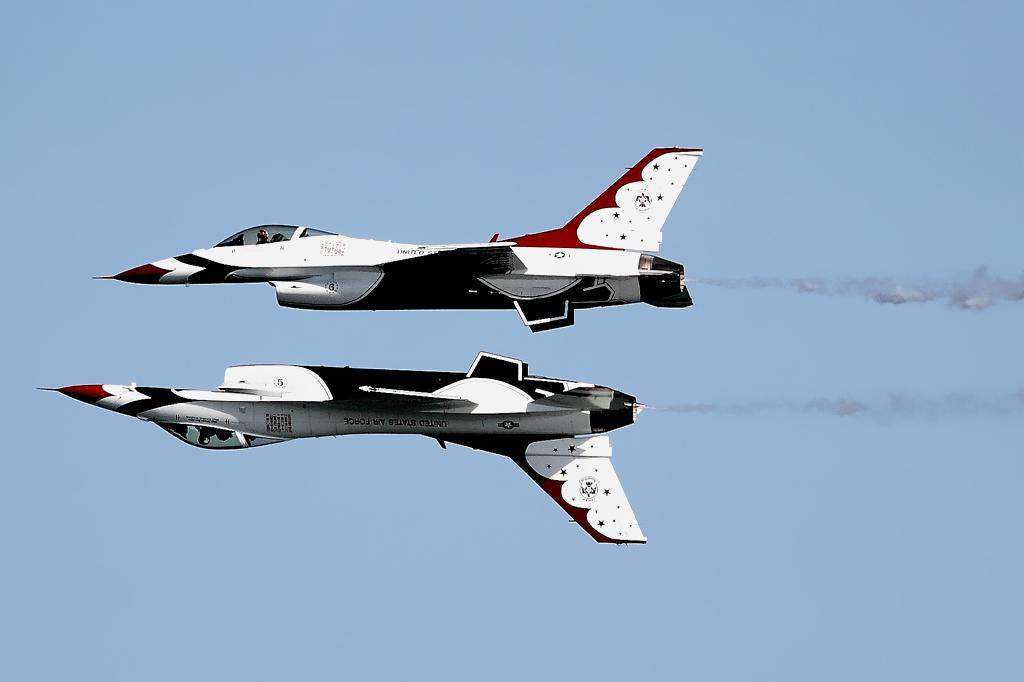
\includegraphics[width=0.49\textwidth]{Wrong-Bernouilli}
\caption{\label{fig:1} The pressure difference just don't count that much in lift}
\end{figure}

\begin{CJK*}{UTF8}{gbsn}
 
\section{前言}
在该第一部分中的一些额外的元素可以被添加。巴贝尔包将采取的翻译服务.

\section{关于数学部分}
在本节中的一些数学会使用数学模型含中文字符显示。
 
\end{CJK*}

Have a look at Fig\ref{fig:1}, trival isn't it?! In reality, lift created by this pressure difference is minor. Whereas a Newton's law seem to apply when taking the flow over airfoil as a whole : the fluid is derived by airfoil {\it somehow (actually by coanda effect)} getting a momentum downwards thus giving airplane a momentum upwards.\\

When angle of attack is not steep (too big), the fluid seems to be tamed and derived downwards passing by airfoil.\\

Slats and flags are used when the civil plane is taking off or landing in order to enhance the coanda effect thus enhance lifts. Fighters do that to cruise at lower speed favoring a quick turn.


\section{Annexe : some Eqs on momentum changing rate}

The momentum of air in a volume that includes volume of the airfoil at instant $t$ (assuming $\rho$ is constant and flow is stationnary for now, so the change will only come from flux/convection):
$$\vec{p} = \iiint_V \rho\vec{v}(\vec{x}) d\tau$$
At $t+\Delta t$
$$\vec{p'} = \iiint_V \rho\vec{v}(\vec{x}) d\tau$$
Momentum change rate:
$$\vec{F}=\frac{d\vec{p}}{dt}= \lim_{\Delta t \to 0} \iiint_V \rho (\frac{\vec{v}(\vec{x}+\vec{v}\Delta t) - \vec{v}(\vec{x})}{\Delta t}) d\tau$$
Which is a direction derivative of $\vec{v}$ in direction $\vec{v}$ (See Pauly's Geometrie 2):
$$\frac{d\vec{p}}{dt}= \iiint_V \rho(\vec{v} \cdot \vec{\nabla} \vec{v}) d\tau$$
Taking the instationnarity into account, we obtain then
$$\frac{d\vec{p}}{dt}= \iiint_V \rho(\frac{\partial\vec{v}}{\partial t} + \vec{v} \cdot \vec{\nabla} \vec{v}) d\tau = \iiint_V \rho \frac{D\vec{v}}{Dt} d\tau$$
Where a total derivative $\frac{d}{dt}$ or material derivative $\frac{D}{Dt}$ is applied. \\

Take one step back and think of Newton's second law in high school which only involves one derivative $\frac{d}{dt}$ which is Lagrangian. Here in fluid mechanics we have total derivative $\frac{d}{dt}$ or material derivative $\frac{D}{Dt}$ for a control volume which is itself static in the case above (if not, Reynolds Theorem applies where the time variation of the control volume is taken into account). What differentiate from high school material point mechanics and fluid mechanics is the presence of flux in and flux out. Mathmatically speaking, we interprate material point with Lagrangian representation and flow with Eularian representation : the $\frac{d}{dt}$ in high school is indeed a material derivative in term of material though there's no flux; $\frac{d}{dt}$ or $\frac{D}{Dt}$ in fluid mechanics are always applied to volumes instead of material points (which is consistent, because $\Delta \tau$ is small but remains a volume) though very often called "fluid particles". And $\frac{Du}{Dt}$ is a Lagrangian quantity (Lagrangian accelaration) dependant on a Eularian variable. $u(\vec{x},t)$. {\bf So in one word, N-S equation is a Lagrangian Newton's second law translated in Eularian variables which as a consequence involves convective/nonlinear term}.\\

A note on vectorial derivative : differentiable function admits vectorial devrivative. 
$$(vf)_a = f_{*,a}(v)=v_1 \frac{\partial f}{\partial x_1}+\dots + v_n \frac{\partial f}{\partial x_n}$$

On Pauly's Geometrie 2. Page 14 and 15. The "tangent space" (maybe 2D and 1D) of two examples are :
$$f(a) + J(f)_a \cdot \left(\begin{array}{c} \lambda_1 \\ \lambda_2 \end{array}\right)$$
and 
$$f(0) + J(f)_0 \cdot (t) = \left(\begin{array}{c} 1/2 t \\ 1/2 t \end{array}\right)$$
$$f(\pi) + J(f)_{\pi} \cdot (t) = \left(\begin{array}{c} -1/2 t \\ 1/2 t \end{array}\right)$$

\newpage
\bibliography{HowPlanesFly}
\bibliographystyle{ieeetr}

\end{document}
